\documentclass[12pt,a4paper]{article}

% Paketi
\usepackage[utf8]{inputenc}
\usepackage[T1]{fontenc}
\usepackage[serbian]{babel}
\usepackage{amsmath}
\usepackage{graphicx}
\usepackage{booktabs}
\usepackage{hyperref}
\usepackage{geometry}
\usepackage{fancyhdr}
\usepackage{listings}
\usepackage{xcolor}
\usepackage{float}

% Slike se traže u oba foldera
\graphicspath{{./figures/}{./notebooks/}}

% Margine
\geometry{a4paper, margin=2.5cm}

% Header i footer
\pagestyle{fancy}
\fancyhf{}
\rhead{\thepage}
\lhead{Klasifikacija gramatičkih facijalnih ekspresija}

% Naslov
\title{
    \Large \textbf{Matematički fakultet, Univerzitet u Beogradu} \\[0.5cm]
    \large Seminarski rad iz predmeta: Istraživanje podataka 2 \\[1cm]
    \LARGE \textbf{Klasifikacija gramatičkih facijalnih ekspresija} \\[0.5cm]
    \large Poređenje algoritama klasifikacije na 3D facial landmarks podacima
}
\author{
    Autor: Zarija Trtović\\
    Broj indeksa: 39/2020 \\[0.5cm]
    Profesor: Mirjana Maljković Ružičić
}
\date{April 2026.}

\begin{document}

\maketitle
\thispagestyle{empty}
\newpage

\tableofcontents
\newpage

% =====================================================
\section{Tekst zadatka}

Zadatak seminarskog rada je klasifikacija \textbf{gramatičkih facijalnih ekspresija} iz istoimenog skupa podataka sa UCI repozitorijuma. Potrebno je:

\begin{itemize}
    \item izvršiti preprocesiranje podataka,
    \item primeniti \textbf{minimum 5 algoritama klasifikacije},
    \item napraviti modele sa \textbf{svim atributima} i sa \textbf{različitim redukovanim skupovima atributa} i uporediti ih,
    \item u skupu u kom ima smisla koristiti \textbf{različite ciljne atribute} i napraviti modele za svaki od njih,
    \item vizuelno prikazati podatke (2D/3D),
    \item izvršiti analizu rezultata i uporediti dobijena rešenja.
\end{itemize}

Rad je realizovan u Python-u uz biblioteku \texttt{scikit-learn}. Sav kod se nalazi u notebook-u \texttt{notebooks/facial\_expressions.ipynb}, a svi rezultati, figure i sačuvani modeli se automatski generišu pri izvršavanju.

% =====================================================
\section{Opis podataka}

\subsection{Izvor i struktura}

Skup podataka \textit{Grammatical Facial Expressions} potiče sa UCI Machine Learning Repository. Podaci su dobijeni sa \textit{Microsoft Kinect} senzora i sadrže \textbf{3D koordinate 100 tačaka lica} (facial landmarks) tokom izvođenja gramatičkih facijalnih ekspresija u brazilskom znakovnom jeziku (LIBRAS).

\begin{itemize}
    \item \textbf{18 \textit{datapoints} fajlova}: svaki red = jedan frame, 301 kolona (timestamp + 100$\times$3 koordinate).
    \item \textbf{18 \textit{targets} fajlova}: binarne oznake (0 = neaktivna, 1 = aktivna) za svaki frame.
    \item Imenovanje fajlova: \texttt{[korisnik]\_[ekspresija]\_datapoints.txt}.
    \item Korisnici: \textbf{A} i \textbf{B} (dva subjekta).
    \item Ekspresije (9): \textit{affirmative, conditional, doubt\_question, emphasis, negative, relative, topics, wh\_question, yn\_question}.
\end{itemize}

\subsection{Osnovna statistika}

\begin{table}[H]
\centering
\begin{tabular}{lc}
\toprule
\textbf{Metrika} & \textbf{Vrednost} \\
\midrule
Ukupno frame-ova & 27\,936 \\
Broj atributa (feature-a) & 300 \\
Broj korisnika & 2 (A: 13\,610, B: 14\,326) \\
Broj tipova ekspresija & 9 \\
Distribucija labela (0/1) & 18\,059 / 9\,877 \\
Procenat aktivnih (label=1) & 35{,}36\,\% \\
Nedostajućih vrednosti & 0 \\
\bottomrule
\end{tabular}
\caption{Osnovna statistika dataseta pre preprocesiranja.}
\end{table}

\subsection{Vizualizacija}

Distribucija klasa i primer 3D rekonstrukcije jednog frame-a prikazani su na slikama \ref{fig:dist} i \ref{fig:3d}.

\begin{figure}[H]
\centering
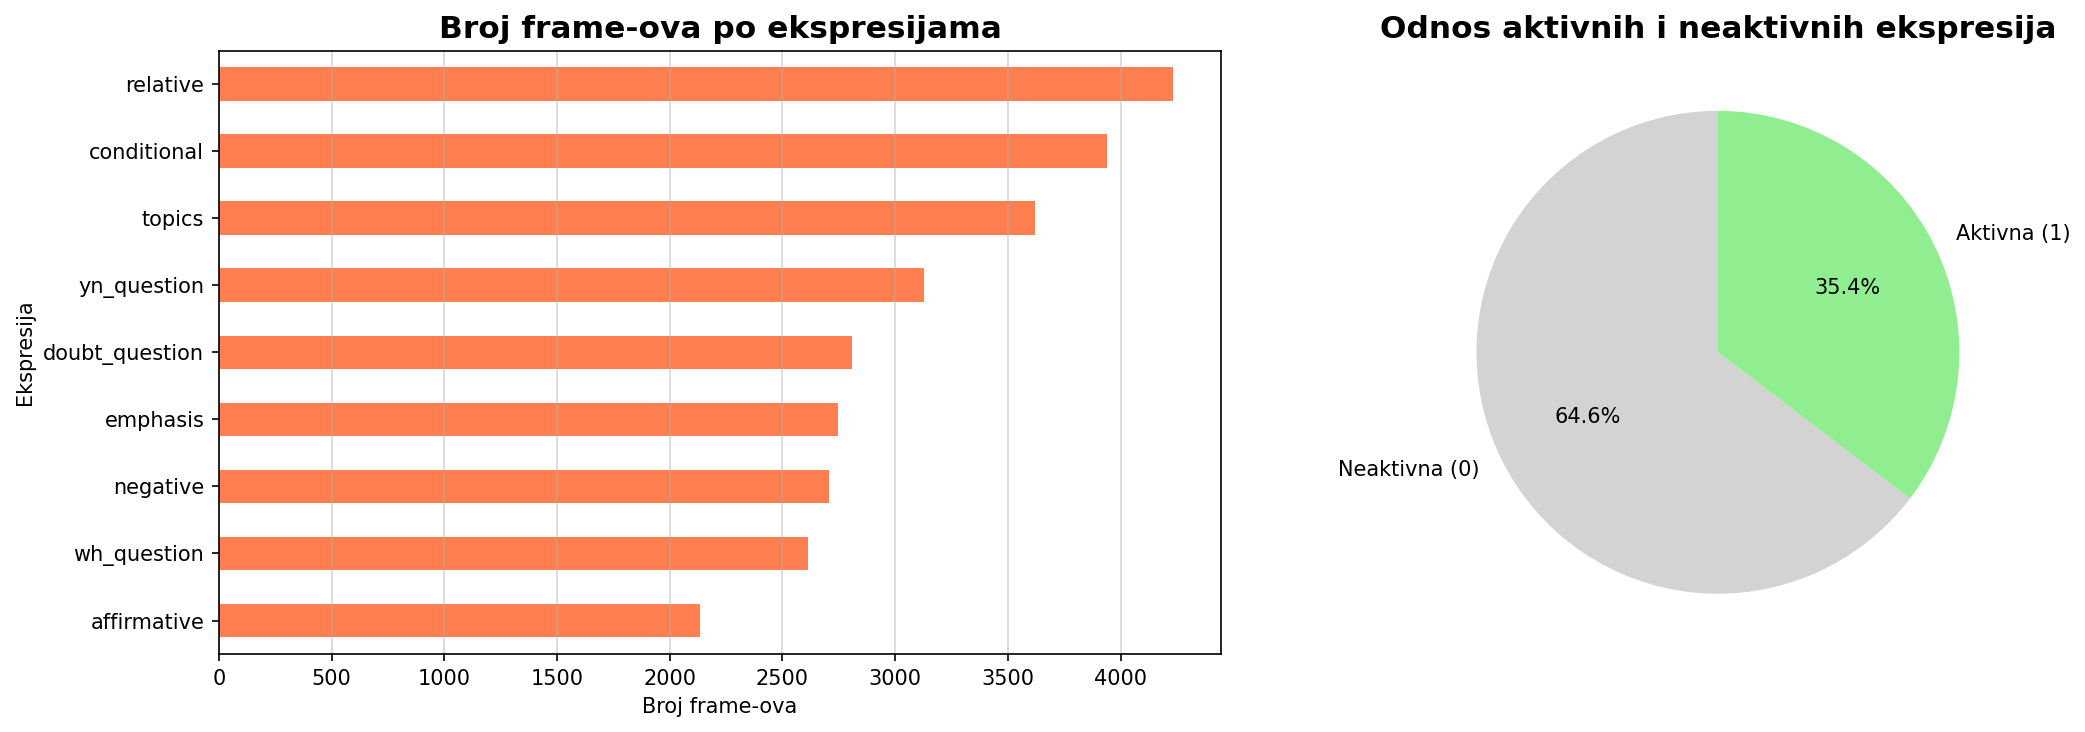
\includegraphics[width=\linewidth]{distribucija.png}
\caption{Broj frame-ova po ekspresijama (levo) i odnos aktivnih/neaktivnih frame-ova (desno).}
\label{fig:dist}
\end{figure}

\begin{figure}[H]
\centering
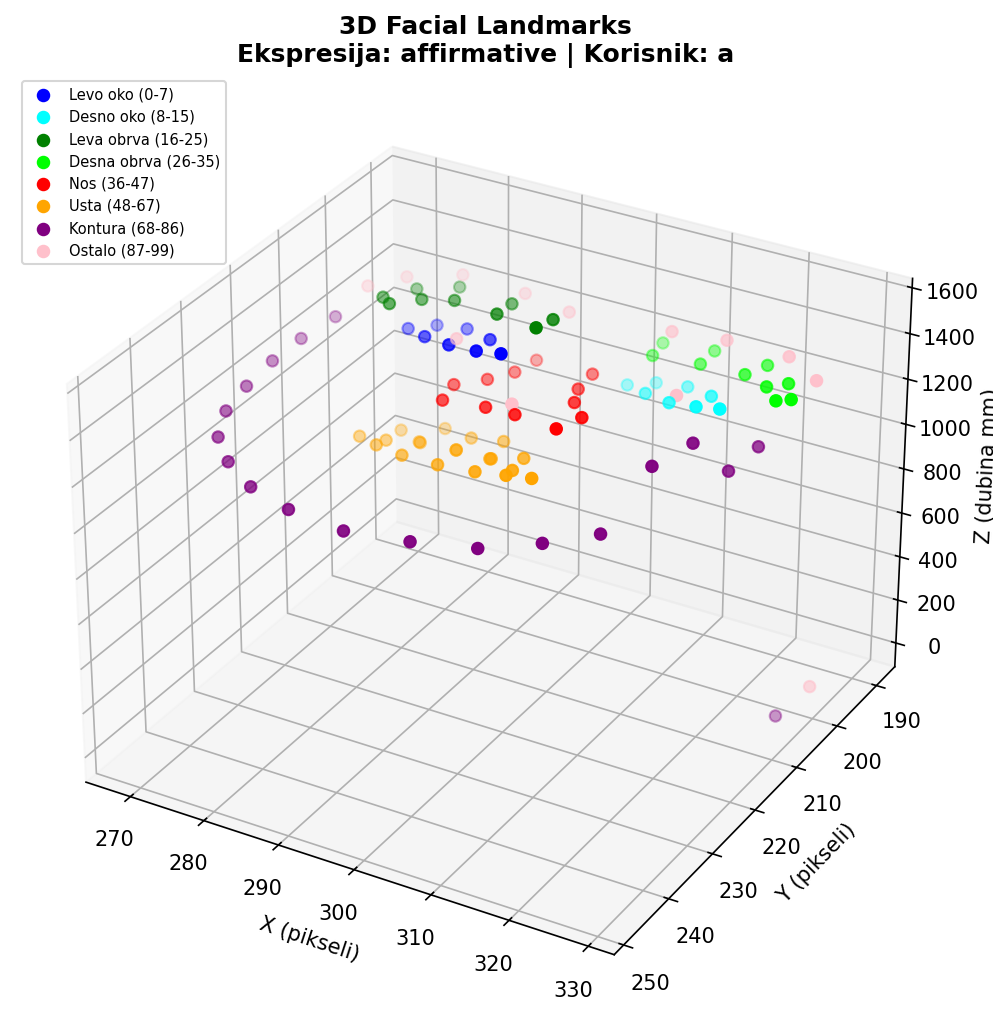
\includegraphics[width=0.75\linewidth]{3d_landmarks.png}
\caption{3D prikaz 100 facial landmarks za jedan frame, grupisanih po delovima lica (oči, obrve, nos, usta, kontura).}
\label{fig:3d}
\end{figure}

% =====================================================
\section{Opis obrade podataka}

\subsection{Učitavanje i spajanje}

Funkcija \texttt{load\_all\_data} parsira svih 18 \textit{datapoints} i 18 \textit{targets} fajlova, dodaje kolone \texttt{user} i \texttt{expression} iz imena fajla i spaja sve u jedan \texttt{DataFrame} oblika \textbf{(27\,936, 304)}.

\subsection{Preprocesiranje (čišćenje)}

\begin{enumerate}
    \item \textbf{Uklanjanje timestamp kolone} -- kolona \texttt{0.0} (vreme snimanja) ne nosi informaciju relevantnu za klasifikaciju.
    \item \textbf{Tretiranje Z=0 vrednosti} -- Kinect ne uspeva uvek da izmeri dubinu, pa unosi vrednost 0. Ove vrednosti su zamenjene \textbf{medijanom te Z-koordinate}. Posle zamene: 0 Z=0 vrednosti, 0 NaN.
    \item \textbf{Čuvanje verzija dataseta} -- \texttt{dataset\_original.csv} i \texttt{dataset\_preprocessed.csv}.
\end{enumerate}

\subsection{Ciljni atributi}

Korišćena su \textbf{dva ciljna atributa} (u skladu sa zahtevom zadatka):

\begin{itemize}
    \item \textbf{Cilj A -- \texttt{expression} (9 klasa):} tip gramatičke ekspresije. Label encoding (\texttt{affirmative}$\to$0, \texttt{conditional}$\to$1, \dots, \texttt{yn\_question}$\to$8).
    \item \textbf{Cilj B -- \texttt{label} (2 klase):} da li je u datom frame-u ekspresija aktivna (1) ili neaktivna (0).
\end{itemize}

\subsection{Train/test split i skaliranje}

\begin{itemize}
    \item \textbf{Train/test split}: 80\,\% / 20\,\%, \texttt{stratify} po ciljnom atributu, \texttt{random\_state=42}. \\
    Train: 22\,348 uzoraka, Test: 5\,588 uzoraka.
    \item \textbf{StandardScaler}: fit \emph{samo na train} setu, transform zatim primenjen na test set (sprečava data leakage). Skaliranje je neophodno jer su X,Y u pikselima ($\sim$200--400) a Z u milimetrima ($\sim$800--1600).
    \item Kreirani su \textbf{odvojeni scaler-i} za cilj A i cilj B.
\end{itemize}

% =====================================================
\section{Redukcija atributa i eksperimenti sa parametrima}

Napravljena su \textbf{tri skupa atributa} koja se koriste u svim daljim modelima:

\begin{enumerate}
    \item \textbf{All\_Features}: svih 300 originalnih atributa.
    \item \textbf{PCA}: broj komponenti odabran eksperimentalno.
    \item \textbf{SelectKBest}: $k$ odabrano eksperimentalno (ANOVA F-test, \texttt{f\_classif}).
\end{enumerate}

Za svaku od ovih tehnika, kao i za algoritme KNN, Decision Tree, MLP i SVM, urađen je poseban \textbf{eksperiment za biranje hiperparametara}.

\subsection{PCA eksperiment}

Testiran broj komponenti: \{10, 20, 30, 50, 75, 100, 150, 200\}. Kao probne modele koristili smo KNN, MLP i SVM na \texttt{expression} cilju.

\begin{figure}[H]
\centering
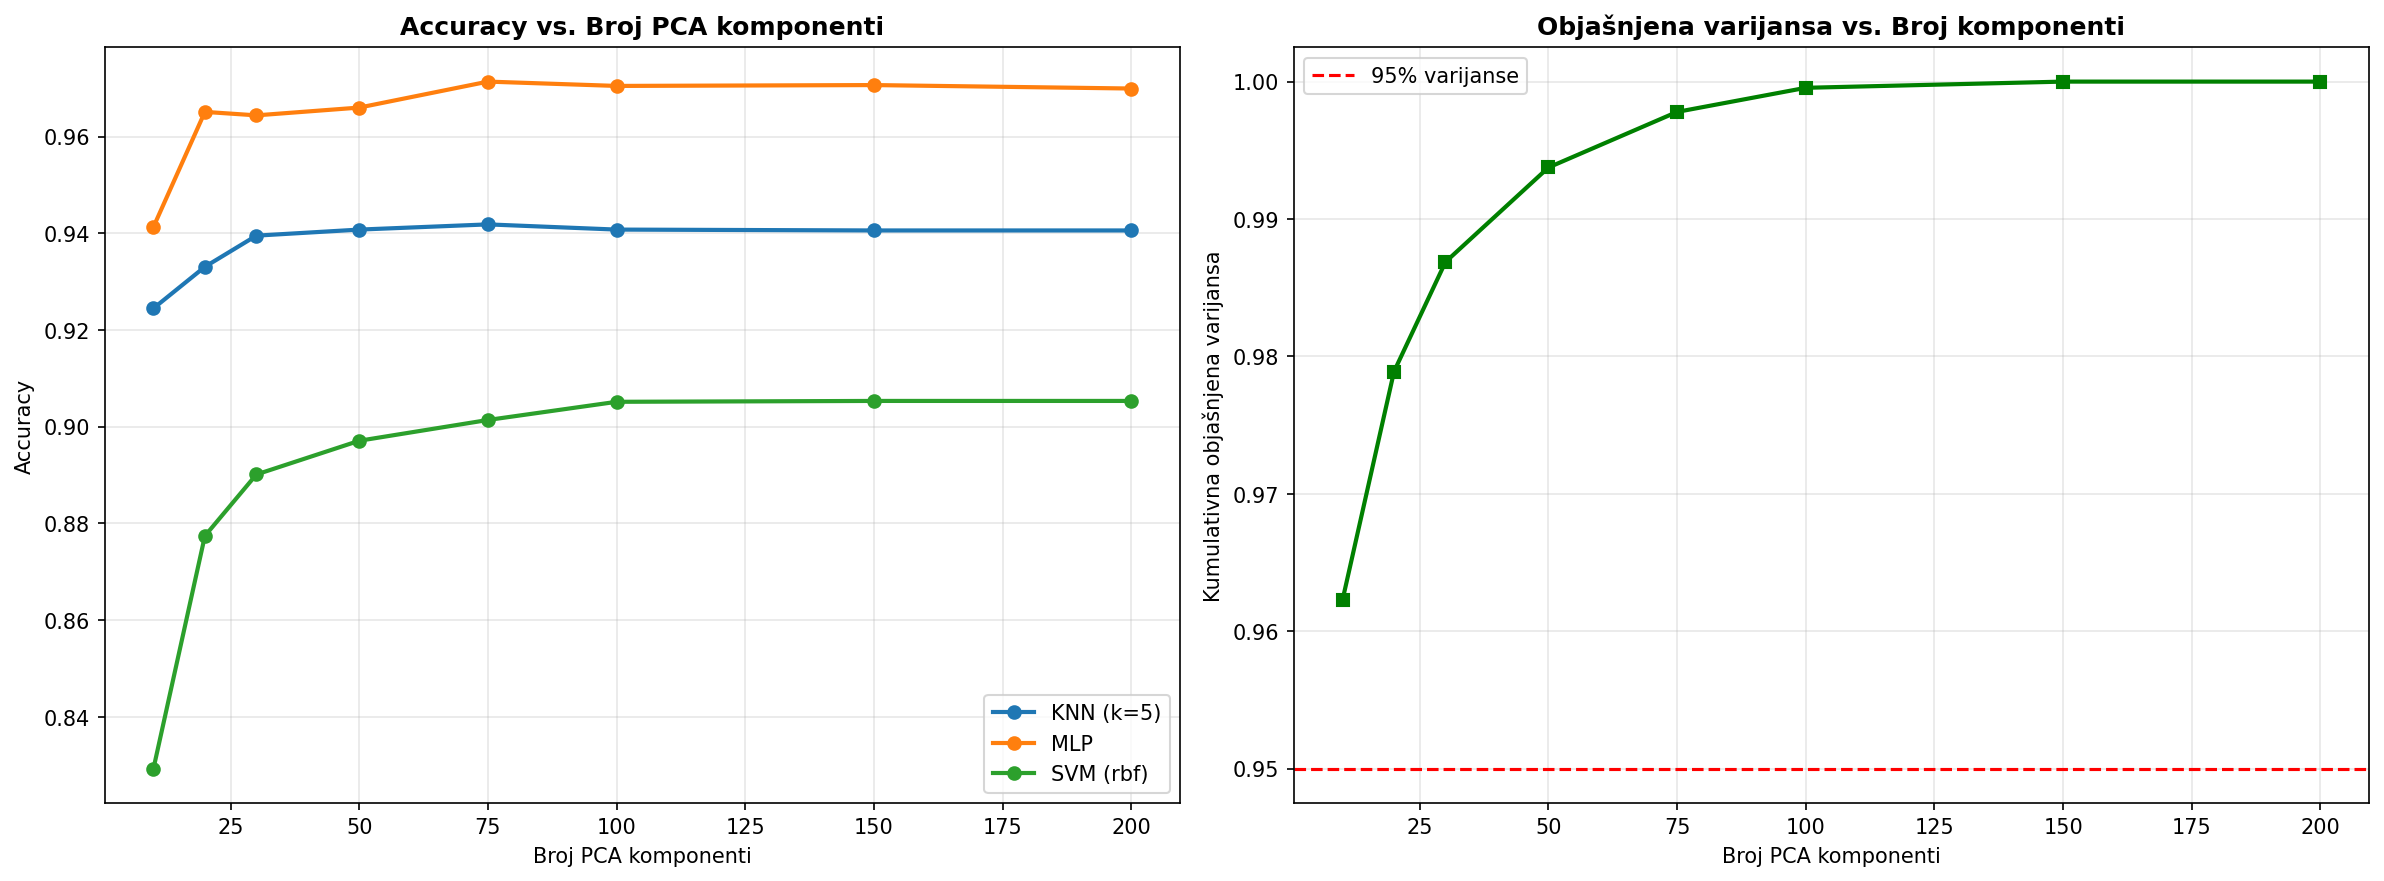
\includegraphics[width=\linewidth]{pca_experiment.png}
\caption{Accuracy vs. broj PCA komponenti (levo) i kumulativna objašnjena varijansa (desno).}
\label{fig:pca}
\end{figure}

\textbf{Rezultat:} optimalno \textbf{PCA(75)} sa MLP dostiže \textbf{Accuracy = 0{,}9714} i objašnjava \textbf{99{,}78\,\%} varijanse. Daljim povećanjem broja komponenti (100, 150, 200) skor stagnira ili opada -- 75 komponenti je dobar trade-off između kompresije i informacije. Ovo se koristi kao PCA skup u daljem radu.

\subsection{SelectKBest eksperiment}

Testiran $k \in \{50, 100, 150\}$.

\begin{figure}[H]
\centering
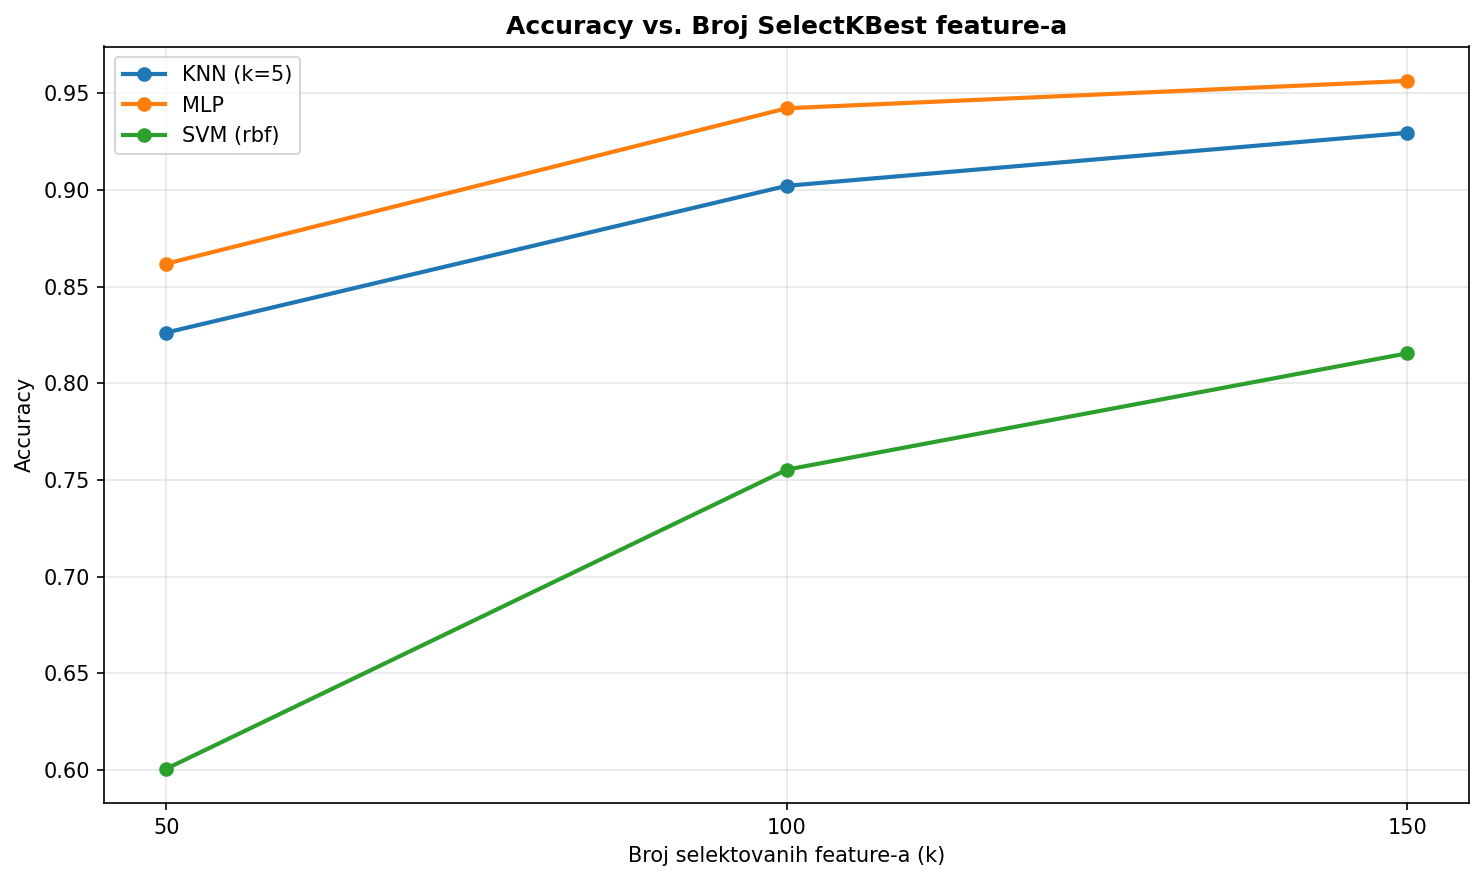
\includegraphics[width=0.75\linewidth]{kbest_experiment.png}
\caption{Accuracy u zavisnosti od broja odabranih feature-a (SelectKBest).}
\label{fig:kbest}
\end{figure}

\textbf{Rezultat:} biramo \textbf{k=100} (MLP Acc=0{,}9422). Iako k=150 daje neznatno bolji skor (MLP Acc=0{,}9563), 100 feature-a daje vrlo slične rezultate uz 50 manje feature-a -- bolji trade-off između performansi i kompleksnosti modela. Top-10 feature-a sa najvećim F-skorom su X-koordinate tačaka oko usta (\texttt{41x, 42x, 52x, 97x, 51x, 98x, 40x, 62x, 50x, 39x}), što je intuitivno jer pokret usta nosi ključne informacije za gramatičke ekspresije.

\subsection{KNN eksperiment -- izbor k}

Testiran $k \in \{1, 3, 5, 7, 11, 15, 21\}$.

\begin{figure}[H]
\centering
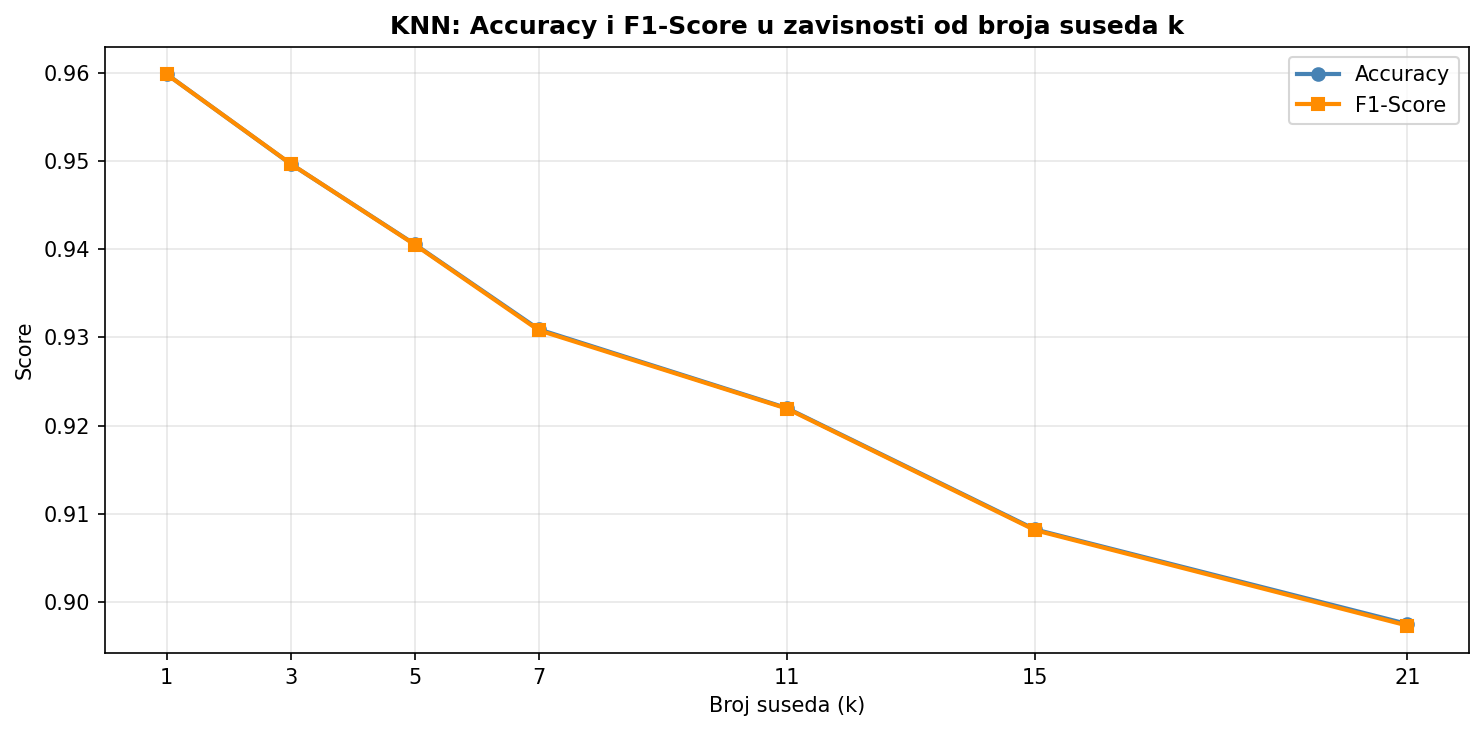
\includegraphics[width=0.75\linewidth]{knn_k_experiment.png}
\caption{Accuracy i F1 KNN-a u funkciji broja suseda.}
\label{fig:knn}
\end{figure}

\textbf{Rezultat:} $k=1$ daje najviši skor (Acc=0{,}9599), ali je podložan šumu. U finalnom treningu koristimo \textbf{k=5} (Acc=0{,}9406) kao robusniji izbor. Dalje povećanje $k$ monotono pogoršava performansu (k=21: Acc=0{,}8975), pošto previše dalekih suseda razvodnjava signal.

\subsection{Decision Tree eksperiment -- max\_depth}

Testirana dubina $\in \{3, 5, 7, 10, 15, 20\}$.

\begin{figure}[H]
\centering
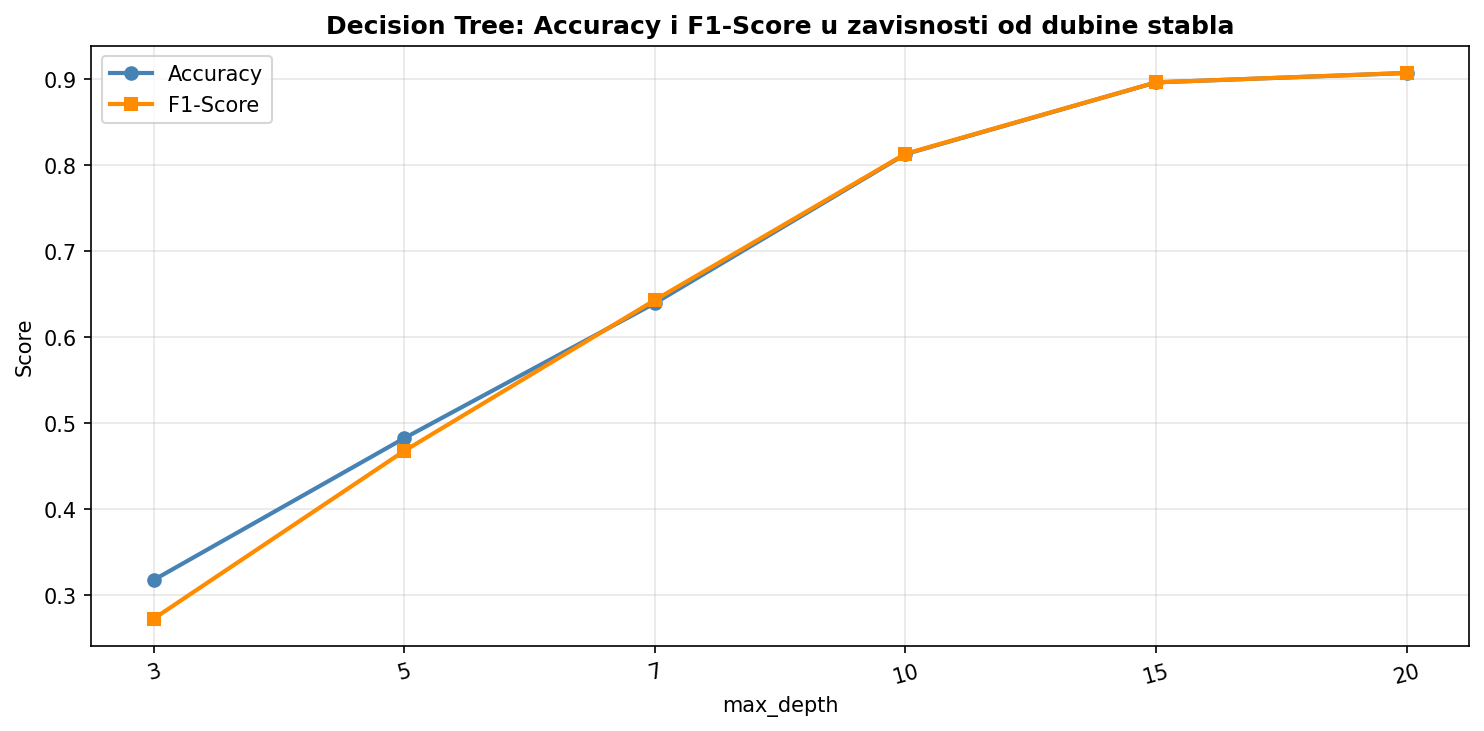
\includegraphics[width=0.75\linewidth]{dt_depth_experiment.png}
\caption{Accuracy i F1 Decision Tree-a u funkciji max\_depth.}
\label{fig:dt}
\end{figure}

\textbf{Rezultat:} accuracy snažno raste sa dubinom: max\_depth=3 daje samo 0{,}3176, max\_depth=15 dostiže 0{,}8960, a max\_depth=20 vrh od 0{,}9069. Za finalni model koristimo \textbf{max\_depth=15} kao kompromis između performanse i rizika od overfitting-a.

\subsection{MLP eksperiment -- arhitektura i aktivacija}

Testirane arhitekture: (50), (100), (100,50), (100,100), (150,100), (200,100,50); aktivacije: \texttt{relu}, \texttt{tanh}.

\begin{figure}[H]
\centering
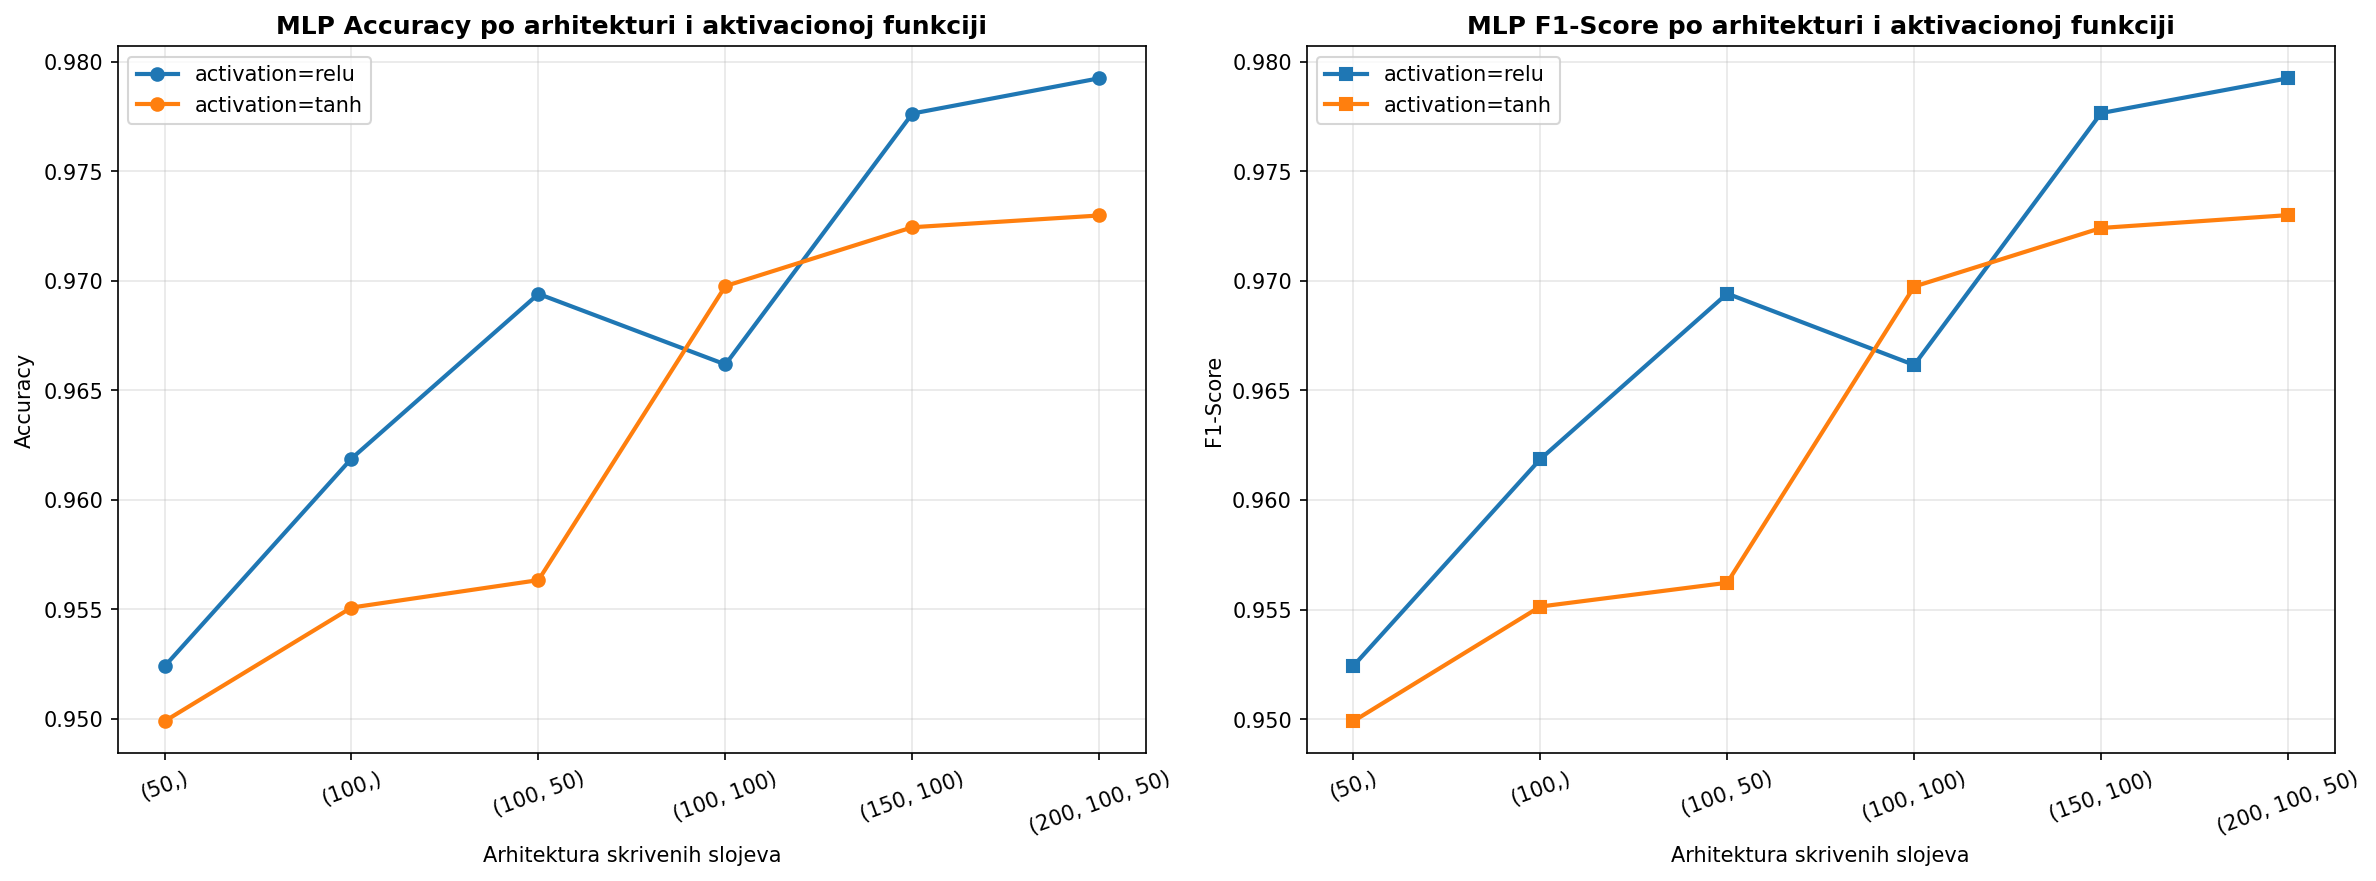
\includegraphics[width=\linewidth]{mlp_architecture_experiment.png}
\caption{MLP Accuracy i F1 po arhitekturi i aktivacionoj funkciji.}
\label{fig:mlp}
\end{figure}

\textbf{Rezultat:} najbolji skor postiže \textbf{(200, 100, 50)} arhitektura -- relu daje Acc=0{,}9792, a tanh Acc=0{,}9730. Performansa uglavnom raste sa kapacitetom mreže, bez znakova overfitting-a. U glavnom eksperimentu koristi se \textbf{(200, 100, 50) + tanh}: iako je u ovom eksperimentu (na svih 300 atributa) relu neznatno bolji, u kombinaciji sa PCA(75) tanh se pokazao kao stabilniji izbor i daje najbolji ukupan rezultat (Acc=0{,}9817, vidi tabelu \ref{tab:top}).

\subsection{SVM eksperiment -- kernel}

Testirani kerneli: \texttt{linear, rbf, poly, sigmoid}.

\begin{figure}[H]
\centering
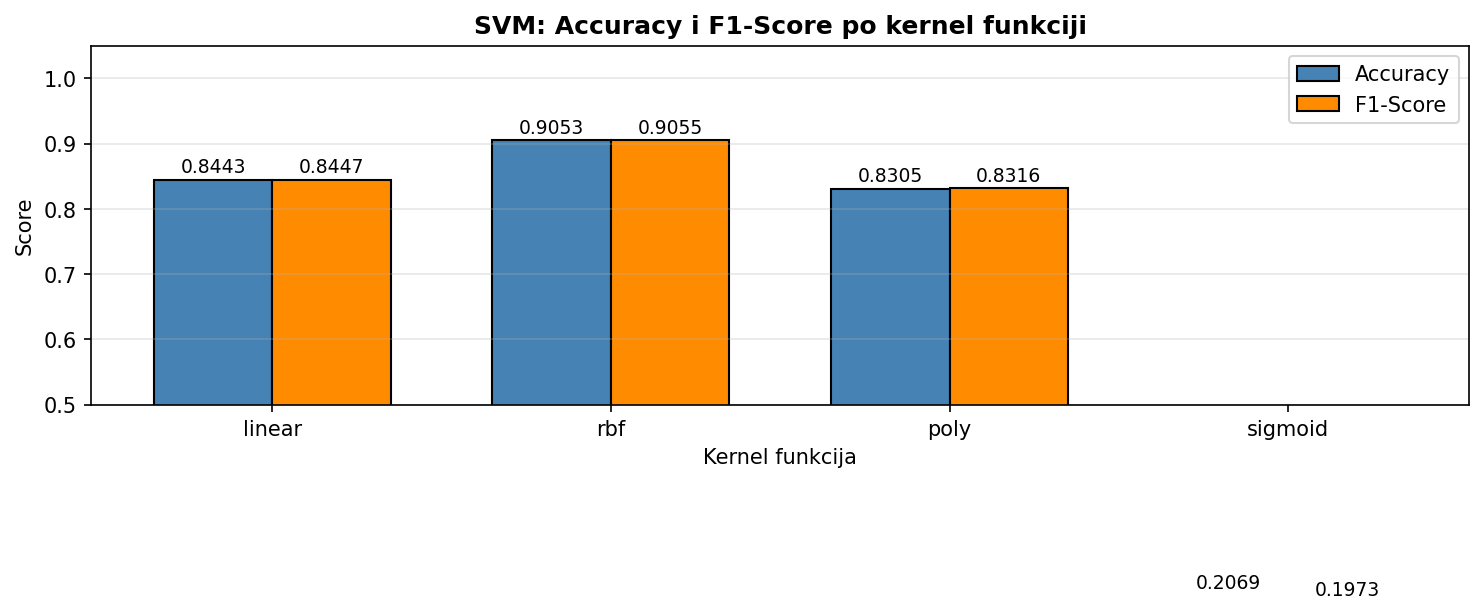
\includegraphics[width=0.75\linewidth]{svm_kernel_experiment.png}
\caption{SVM Accuracy i F1 po kernel funkciji.}
\label{fig:svm}
\end{figure}

\textbf{Rezultat:} \textbf{rbf} kernel je najbolji (Acc=0{,}9053), \texttt{linear} (0{,}8443) i \texttt{poly} (0{,}8305) značajno zaostaju, a \texttt{sigmoid} se pokazao kao neupotrebljiv (Acc=0{,}2069). Ovo potvrđuje da je granica između klasa \emph{nelinearna}.

% =====================================================
\section{Metod -- algoritmi i evaluacija}

\subsection{Korišćeni algoritmi}

Primenjeno je \textbf{5 algoritama} pokrivajući različite paradigme mašinskog učenja:

\begin{table}[H]
\centering
\begin{tabular}{lp{9cm}}
\toprule
\textbf{Algoritam} & \textbf{Hiperparametri} \\
\midrule
Logistic Regression & \texttt{max\_iter=3000, random\_state=42} \\
K-Nearest Neighbors & \texttt{n\_neighbors=5} \\
Decision Tree & \texttt{max\_depth=15, random\_state=42} \\
Support Vector Machine & \texttt{kernel='rbf', C=1.0, random\_state=42} \\
Neural Network (MLP) & \texttt{hidden\_layer\_sizes=(200, 100, 50), activation='tanh', max\_iter=500} \\
\bottomrule
\end{tabular}
\caption{Finalne konfiguracije modela korišćene u glavnom eksperimentu.}
\end{table}

\subsection{Dizajn eksperimenta}

Svaki od 5 algoritama je treniran na \textbf{3 skupa atributa} (All\_Features, PCA\_75, KBest\_100) i \textbf{2 ciljna atributa} (Expression, Label) -- ukupno $5 \times 3 \times 2 = \mathbf{30}$ modela.

\subsection{Metrike}

Korišćene su standardne metrike: \textbf{Accuracy, Precision, Recall, F1-Score}. Za multi-klasni slučaj (Expression, 9 klasa) koristi se \texttt{weighted average}, za binarni (Label) podrazumevana binarna definicija.

% =====================================================
\section{Rezultati i tumačenje}

\subsection{Top modeli}

\begin{table}[H]
\centering
\small
\begin{tabular}{lllcccc}
\toprule
\textbf{Model} & \textbf{Features} & \textbf{Target} & \textbf{Acc} & \textbf{Prec} & \textbf{Rec} & \textbf{F1} \\
\midrule
Neural Network (MLP) & PCA\_75        & Expression & \textbf{0,9817} & 0,9818 & 0,9817 & 0,9817 \\
Neural Network (MLP) & All\_Features  & Expression & 0,9730 & 0,9731 & 0,9730 & 0,9730 \\
Neural Network (MLP) & KBest\_100     & Expression & 0,9594 & 0,9599 & 0,9594 & 0,9595 \\
K-Nearest Neighbors  & PCA\_75        & Expression & 0,9418 & 0,9422 & 0,9418 & 0,9418 \\
K-Nearest Neighbors  & All\_Features  & Expression & 0,9406 & 0,9410 & 0,9406 & 0,9405 \\
Neural Network (MLP) & All\_Features  & Label      & 0,9401 & 0,9399 & 0,8871 & 0,9128 \\
Neural Network (MLP) & PCA\_75        & Label      & 0,9368 & 0,9220 & 0,8973 & 0,9095 \\
Neural Network (MLP) & KBest\_100     & Label      & 0,9345 & 0,9099 & 0,9044 & 0,9071 \\
K-Nearest Neighbors  & KBest\_100     & Label      & 0,9139 & 0,9082 & 0,8416 & 0,8737 \\
K-Nearest Neighbors  & All\_Features  & Label      & 0,9091 & 0,9064 & 0,8284 & 0,8657 \\
\bottomrule
\end{tabular}
\caption{Top 10 modela sortiranih po Accuracy.}
\label{tab:top}
\end{table}

\subsection{Poređenje algoritama (prosek po svim kombinacijama)}

\begin{table}[H]
\centering
\begin{tabular}{lcccc}
\toprule
\textbf{Algoritam} & \textbf{Accuracy} & \textbf{Precision} & \textbf{Recall} & \textbf{F1} \\
\midrule
Neural Network (MLP)   & 0,9542 & 0,9478 & 0,9338 & 0,9406 \\
K-Nearest Neighbors    & 0,9194 & 0,9176 & 0,8807 & 0,8982 \\
Support Vector Machine & 0,8670 & 0,8727 & 0,8044 & 0,8355 \\
Decision Tree          & 0,8631 & 0,8547 & 0,8155 & 0,8339 \\
Logistic Regression    & 0,7693 & 0,7622 & 0,6821 & 0,7167 \\
\bottomrule
\end{tabular}
\caption{Prosečne performanse po algoritmu (6 kombinacija po algoritmu).}
\end{table}

\subsection{Poređenje feature skupova (prosek po svim modelima)}

\begin{table}[H]
\centering
\begin{tabular}{lcccc}
\toprule
\textbf{Skup atributa} & \textbf{Accuracy} & \textbf{Precision} & \textbf{Recall} & \textbf{F1} \\
\midrule
All\_Features (300) & 0,8964 & 0,8937 & 0,8486 & 0,8697 \\
PCA\_75             & 0,8792 & 0,8746 & 0,8249 & 0,8476 \\
KBest\_100          & 0,8482 & 0,8447 & 0,7964 & 0,8177 \\
\bottomrule
\end{tabular}
\caption{Prosečne performanse po feature setu (10 modela po setu).}
\end{table}

\begin{figure}[H]
\centering
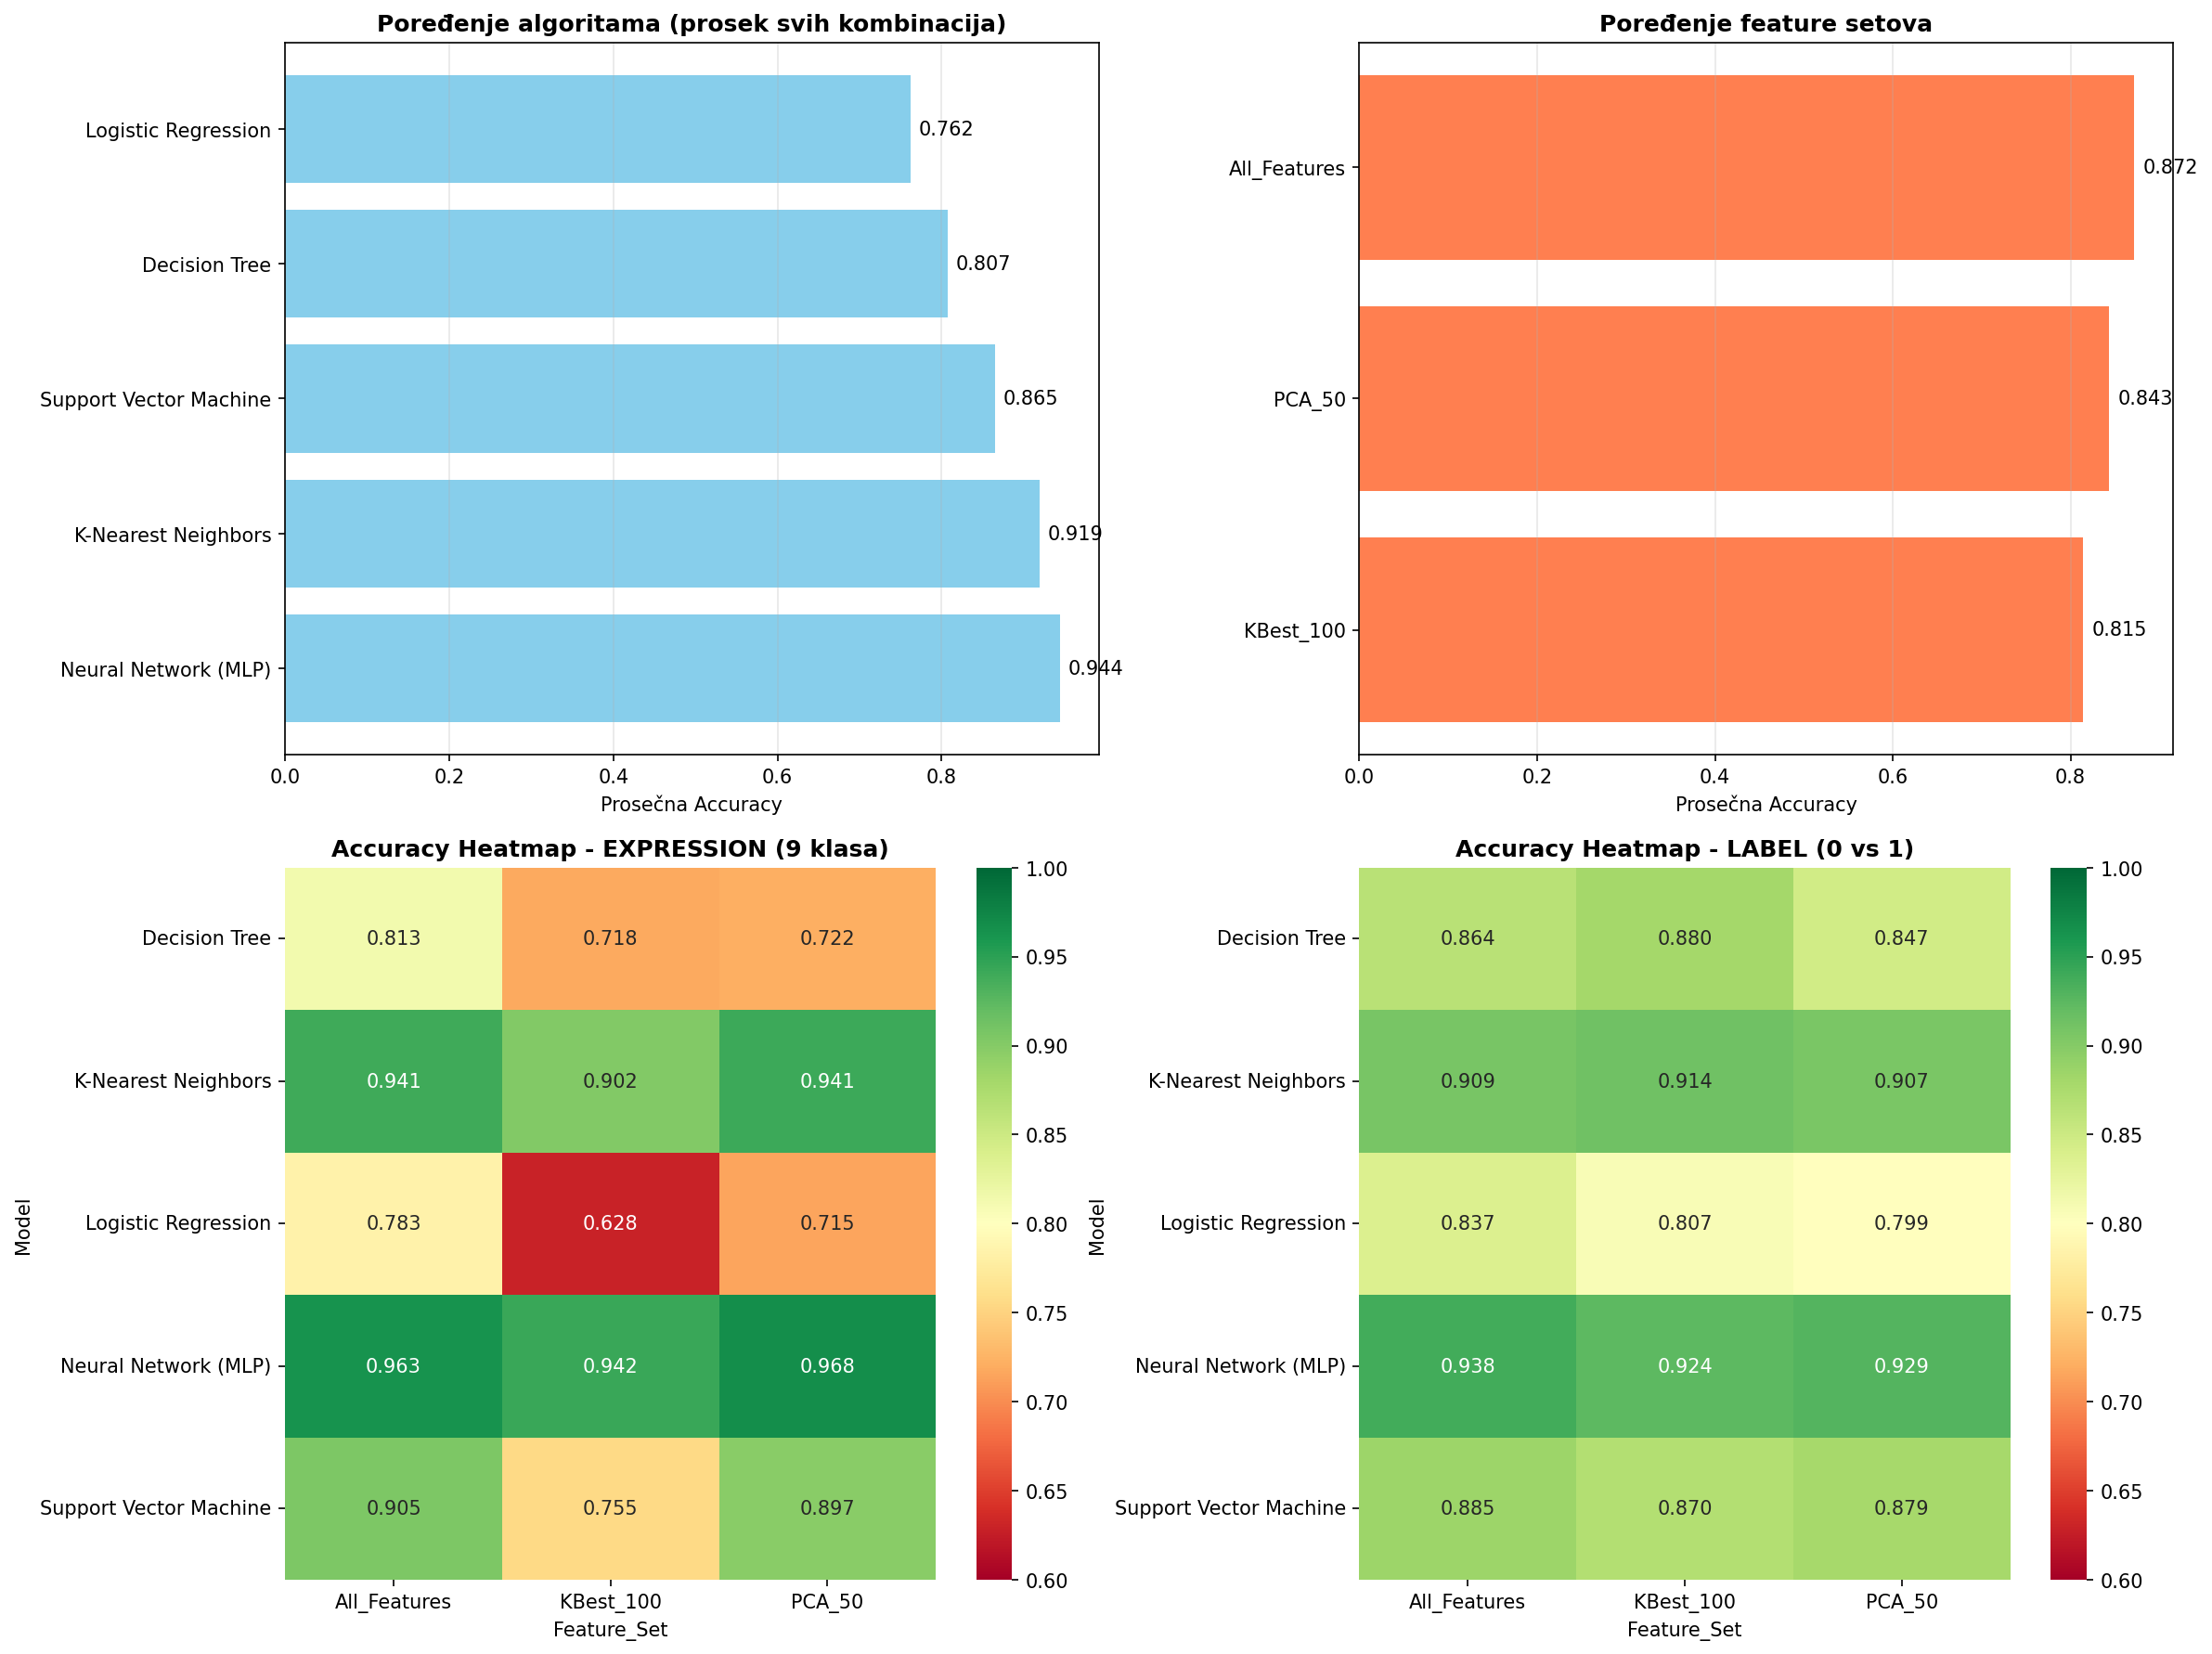
\includegraphics[width=\linewidth]{model_comparison.png}
\caption{Poređenje modela: prosek po algoritmu (gore levo), prosek po feature setu (gore desno) i heatmap po kombinaciji za Expression i Label cilj.}
\label{fig:comp}
\end{figure}

\subsection{Najbolji model -- MLP sa PCA(75), cilj Expression}

\textbf{Accuracy = 0{,}9817} \quad \textbf{F1 = 0{,}9817}

\begin{table}[H]
\centering
\small
\begin{tabular}{lcccc}
\toprule
\textbf{Klasa} & \textbf{Precision} & \textbf{Recall} & \textbf{F1} & \textbf{Support} \\
\midrule
affirmative     & 0,98 & 0,98 & 0,98 & 427 \\
conditional     & 0,98 & 0,98 & 0,98 & 788 \\
doubt\_question & 0,99 & 0,99 & 0,99 & 562 \\
emphasis        & 0,98 & 0,98 & 0,98 & 550 \\
negative        & 0,98 & 0,98 & 0,98 & 541 \\
relative        & 0,98 & 0,98 & 0,98 & 847 \\
topics          & 0,97 & 0,98 & 0,98 & 724 \\
wh\_question    & 0,99 & 1,00 & 0,99 & 523 \\
yn\_question    & 0,99 & 0,97 & 0,98 & 626 \\
\midrule
\textbf{Weighted avg} & \textbf{0,98} & \textbf{0,98} & \textbf{0,98} & \textbf{5588} \\
\bottomrule
\end{tabular}
\caption{Classification report najboljeg modela (MLP + PCA\_75, Expression).}
\end{table}

\begin{figure}[H]
\centering
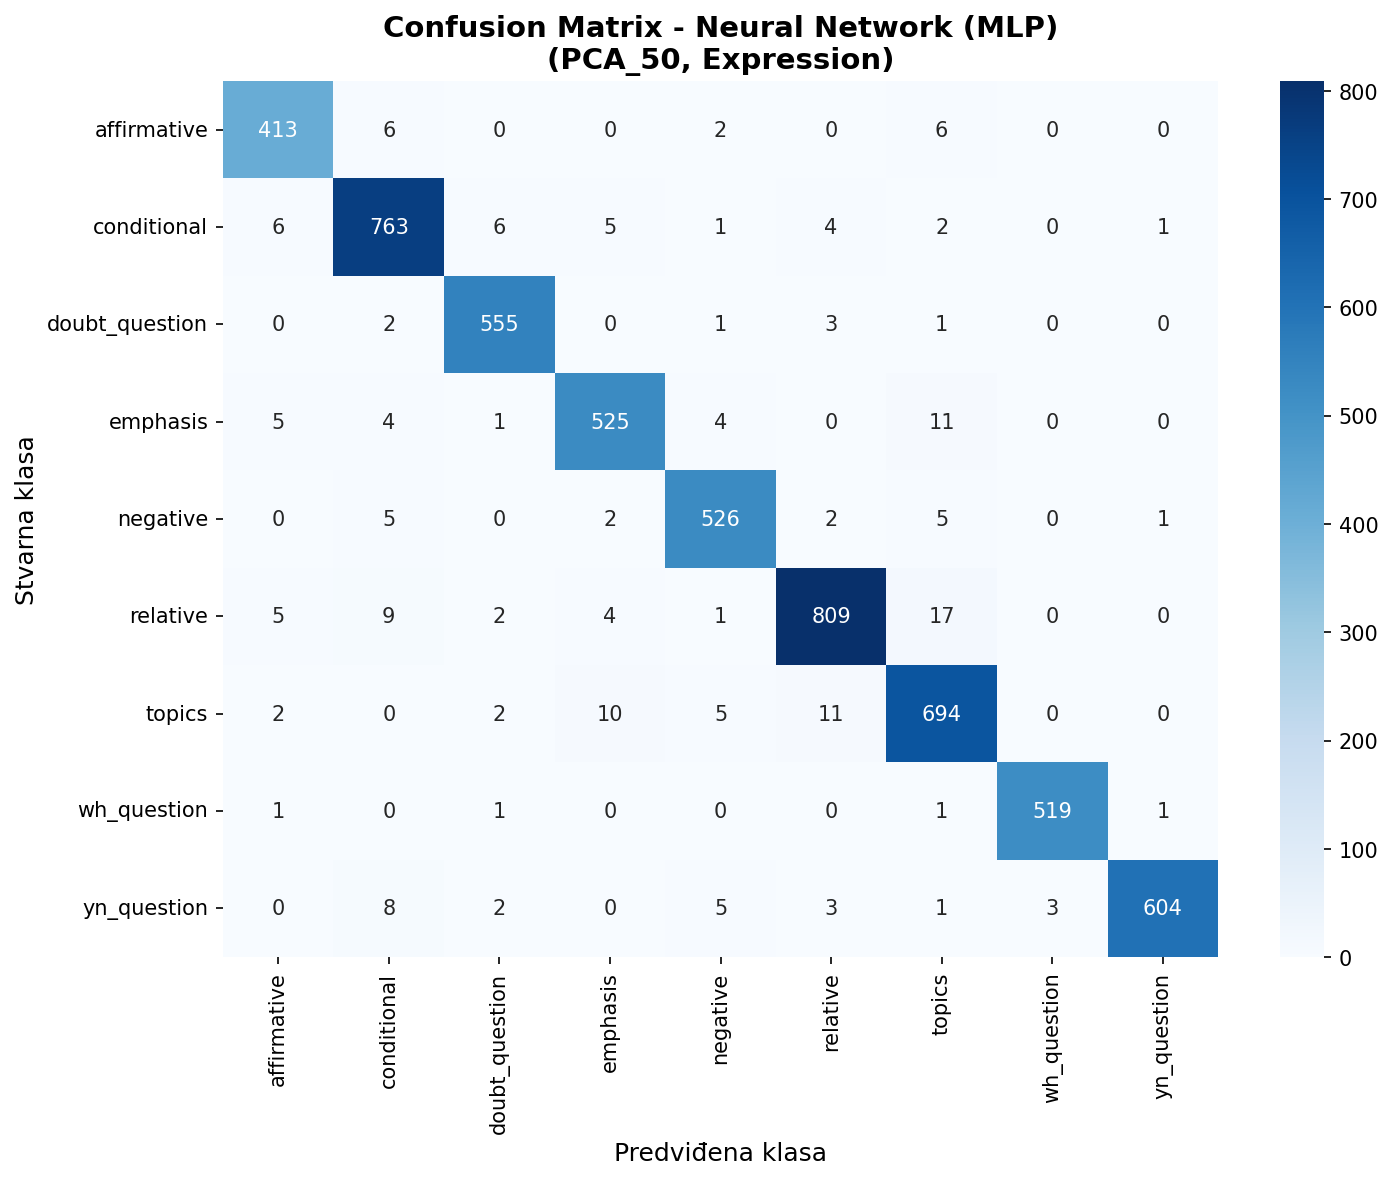
\includegraphics[width=0.8\linewidth]{confusion_matrix_best.png}
\caption{Matrica konfuzije najboljeg modela. Dominira dijagonala; preostale (sitne) greške su ravnomerno raspoređene -- nijedna klasa nije sistematski mešana sa drugom.}
\label{fig:cm}
\end{figure}

\subsection{Per-class analiza i uticaj veličine klase}

Per-class analiza svih 5 algoritama (Expression, All\_Features) prikazana je na slici \ref{fig:perclass}.

\begin{figure}[H]
\centering
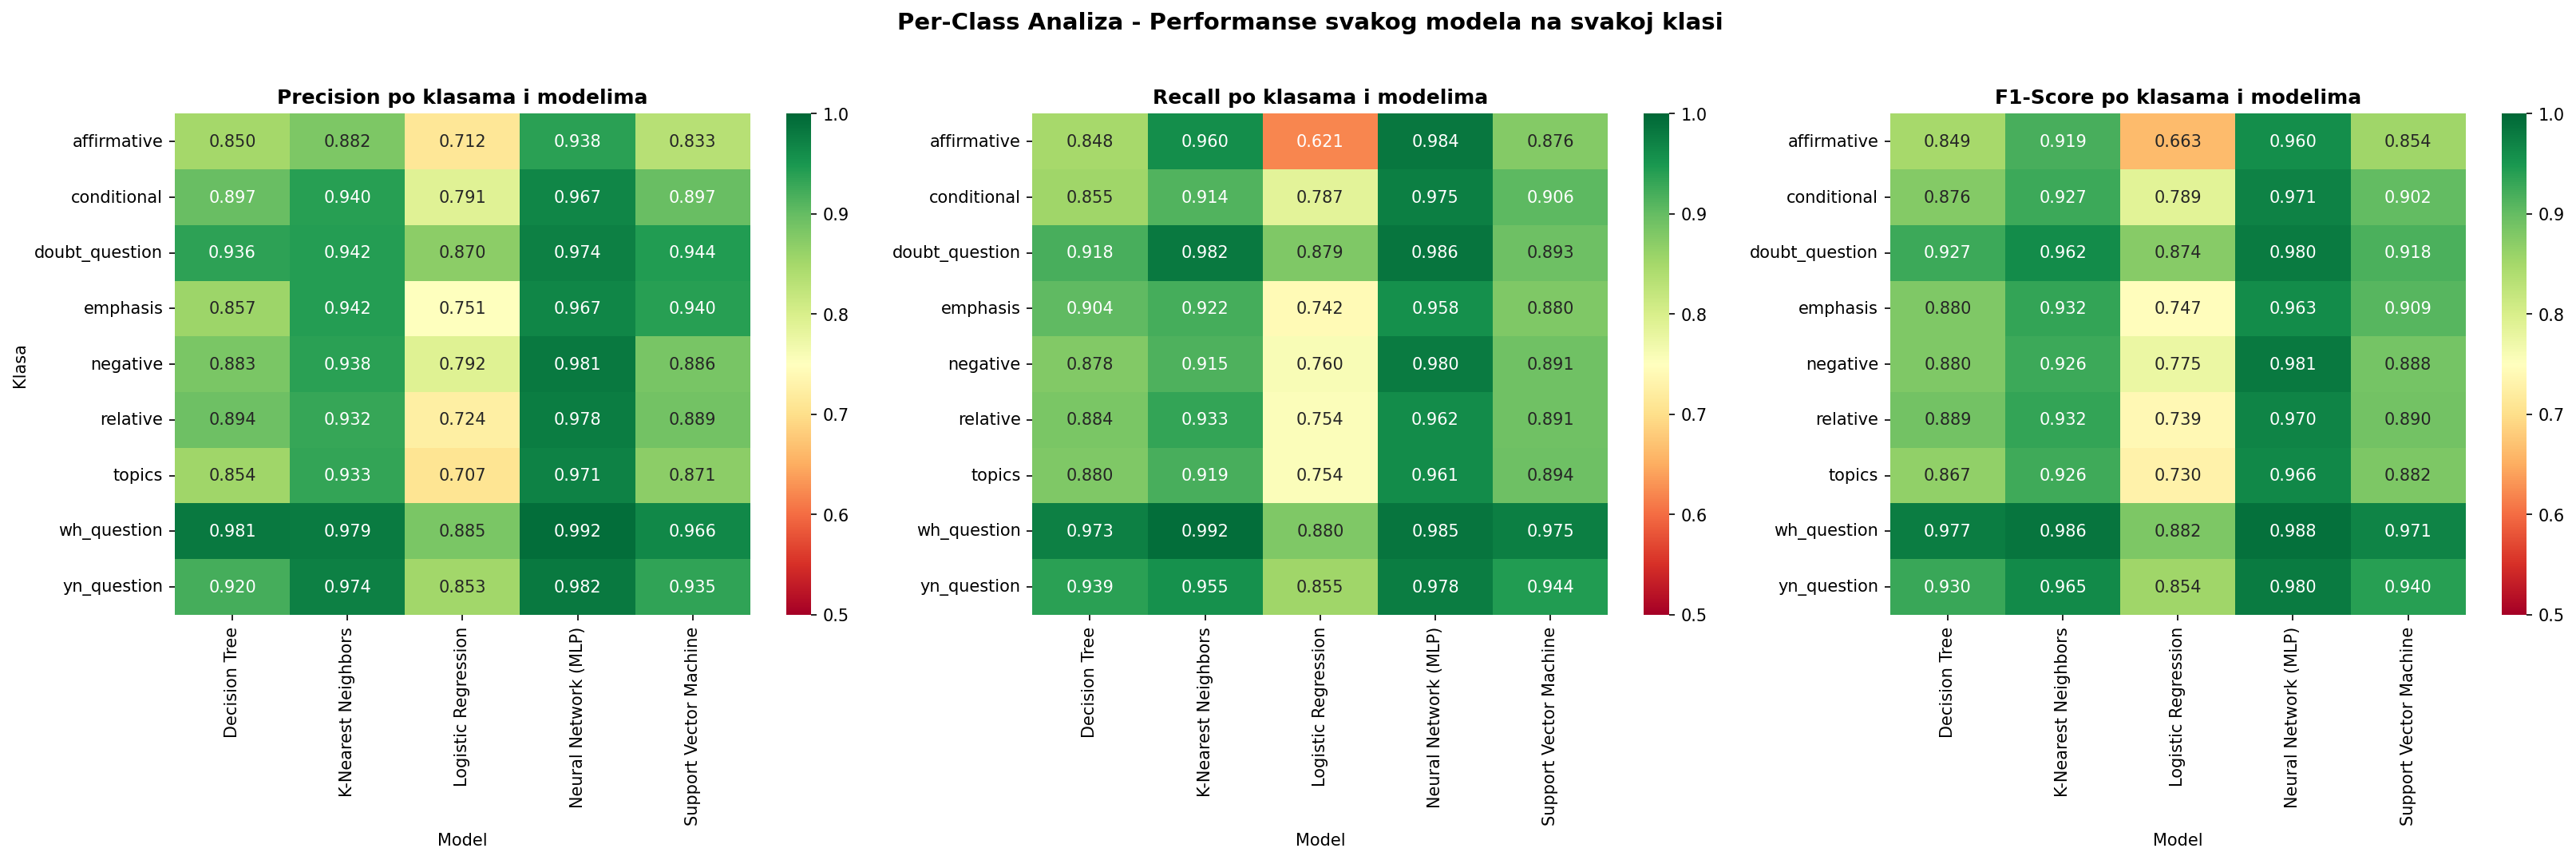
\includegraphics[width=\linewidth]{per_class_analysis.png}
\caption{Heatmap-i Precision, Recall i F1 po klasama i modelima (Expression, All\_Features).}
\label{fig:perclass}
\end{figure}

Glavni nalazi:
\begin{itemize}
    \item Sve klase imaju \textbf{F1 $\geq$ 0{,}92} za MLP i KNN.
    \item \textbf{Logistic Regression} je jedini algoritam sa kombinacijama F1 $<$ 0{,}80 -- za 6 od 9 klasa (npr. \texttt{affirmative} F1=0{,}66, \texttt{topics} F1=0{,}73), što potvrđuje da problem nije linearno separabilan.
    \item \texttt{wh\_question} se najlakše prepoznaje (F1 $\approx$ 0{,}99 kod MLP) jer ima karakteristične pokrete obrva.
\end{itemize}

\paragraph{Uticaj veličine klase.}
Korelacija između broja uzoraka klase i njenog F1 skora kod MLP-a je \textbf{-0{,}087} -- praktično nulta. Najmanja klasa (\texttt{affirmative}, 2\,136 uzoraka) ima F1=0{,}96, najveća (\texttt{relative}, 4\,234 uzoraka) ima F1=0{,}97. \emph{Veličina klase ne utiče značajno na performansu modela}, što potvrđuje da je dataset dovoljno balansiran za ovu analizu.

\begin{figure}[H]
\centering
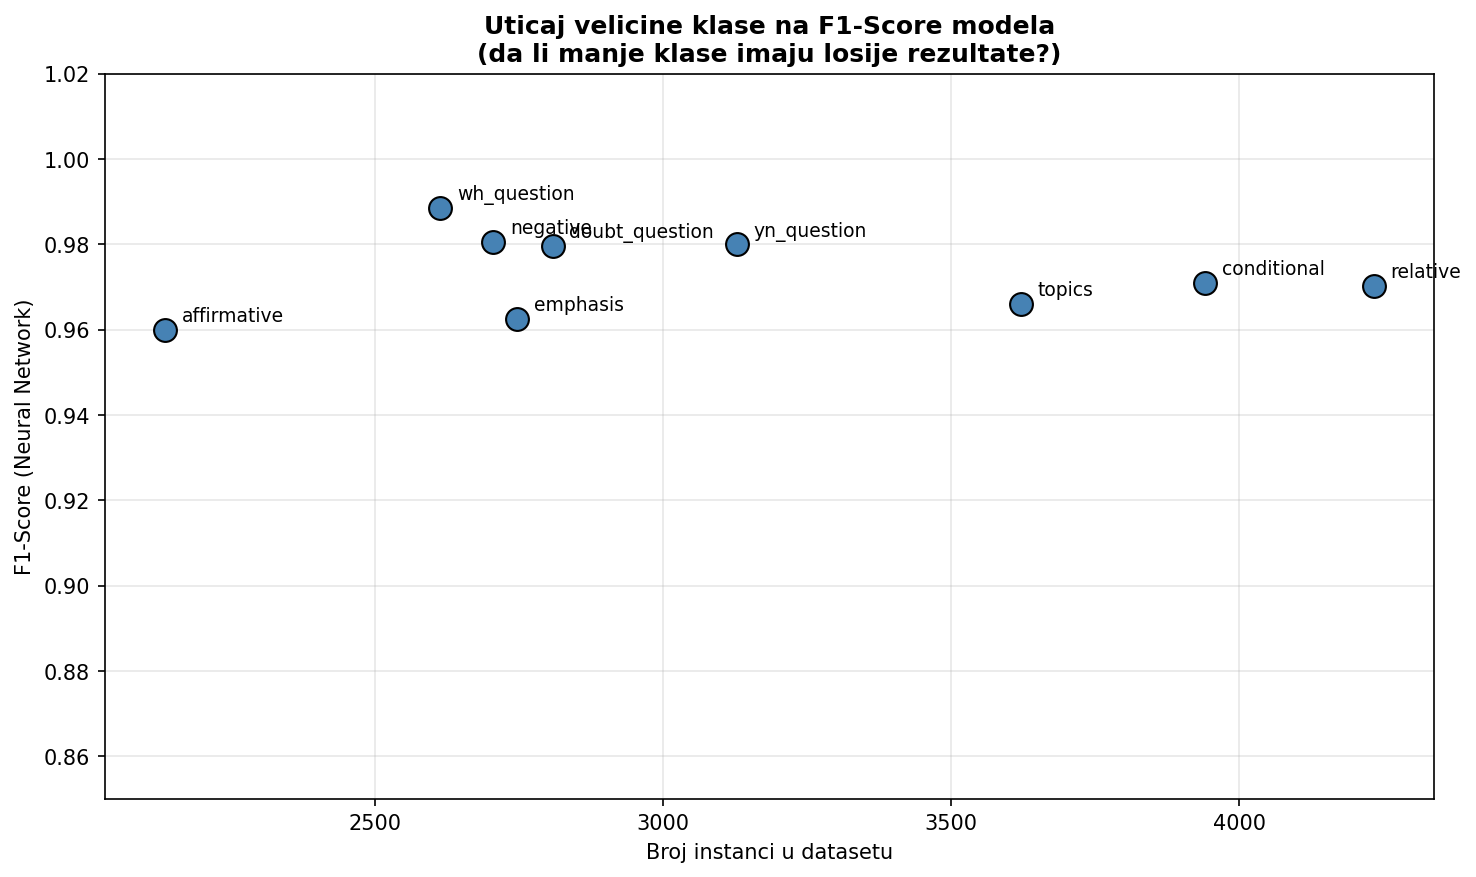
\includegraphics[width=0.7\linewidth]{class_size_vs_f1.png}
\caption{Scatter plot veličine klase vs. F1-Score (Neural Network, All\_Features).}
\label{fig:size}
\end{figure}

\subsection{Confusion matrice za sve modele (Expression, All\_Features)}

\begin{figure}[H]
\centering
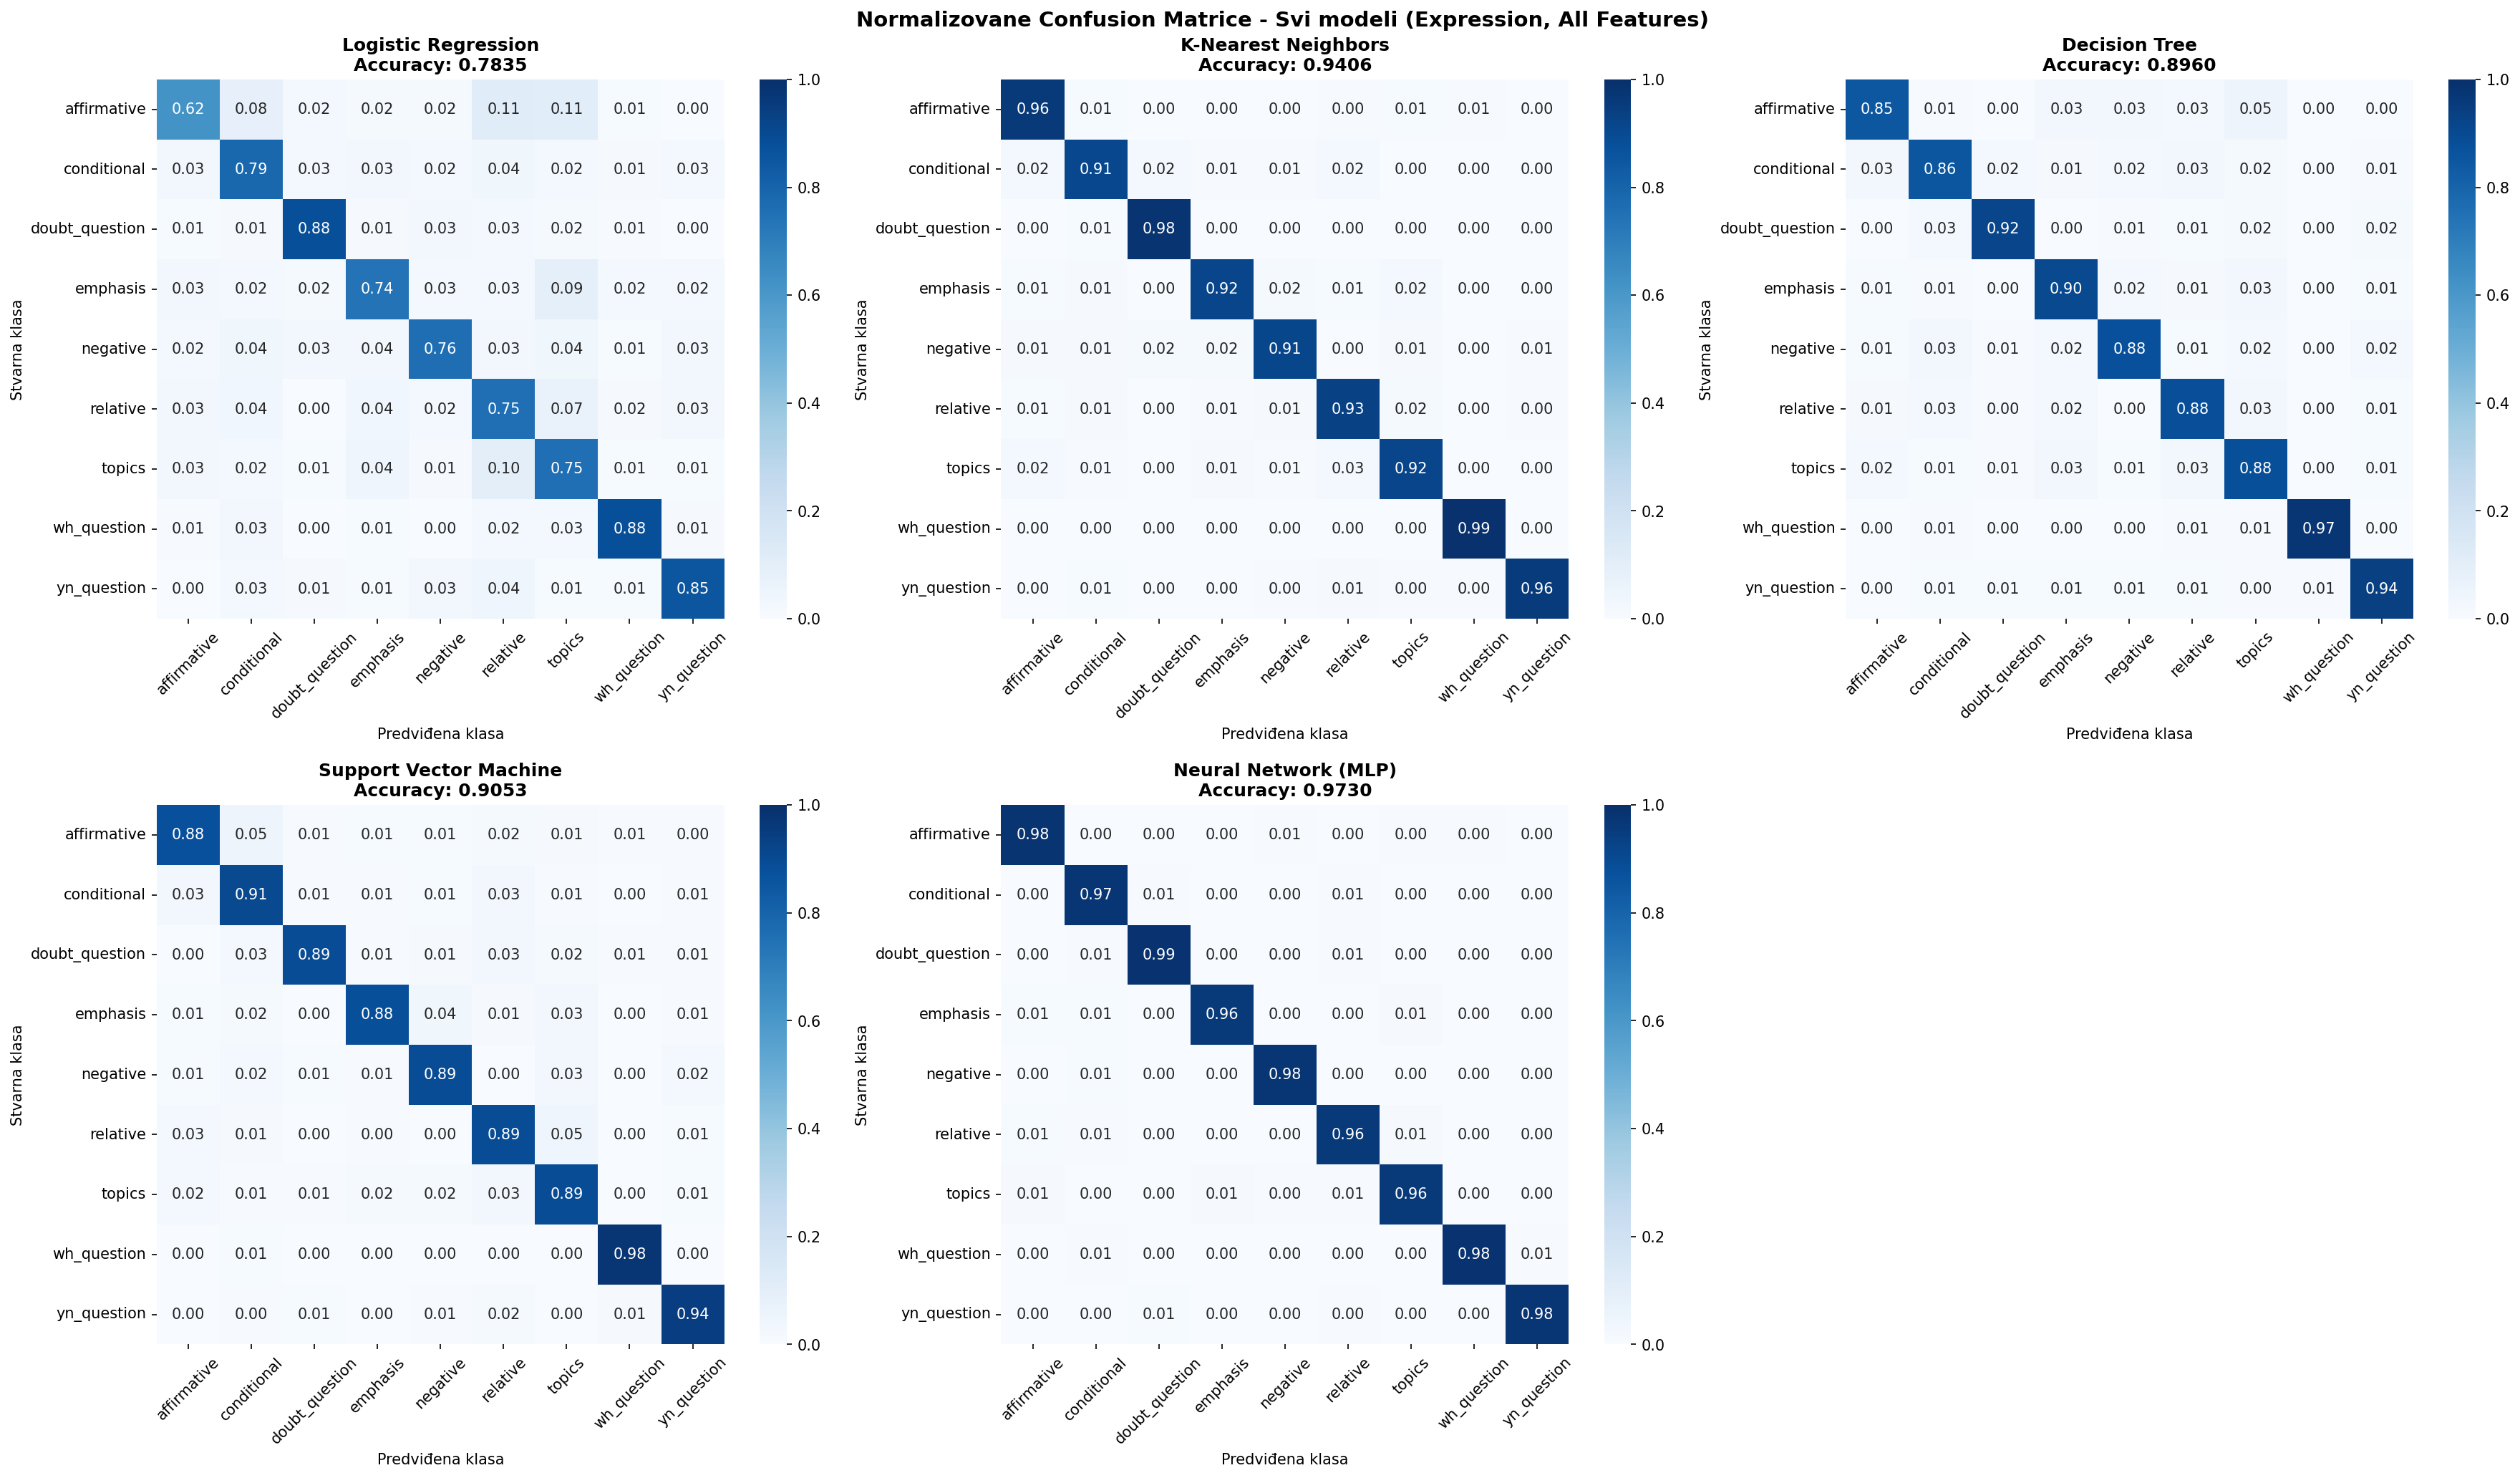
\includegraphics[width=\linewidth]{confusion_matrices_all_models.png}
\caption{Normalizovane matrice konfuzije za svih 5 algoritama. Vidi se da je MLP gotovo savršen, dok kod LR dijagonala bledi -- karakteristične greške su između \textit{affirmative}/\textit{relative} i \textit{topics}/\textit{relative}.}
\label{fig:cm_all}
\end{figure}

\subsection{Label cilj -- binarna klasifikacija aktivna/neaktivna}

Za cilj \texttt{label} (0 vs 1), recall za \emph{aktivnu} klasu (manje zastupljena, 35\,\%) je limitirajući faktor. Vrednosti recall-a za aktivnu klasu po algoritmima (All\_Features):

\begin{table}[H]
\centering
\begin{tabular}{lc}
\toprule
\textbf{Algoritam} & \textbf{Recall (Aktivna)} \\
\midrule
Neural Network (MLP)   & \textbf{0,8871} \\
K-Nearest Neighbors    & 0,8284 \\
Decision Tree          & 0,8153 \\
Support Vector Machine & 0,7642 \\
Logistic Regression    & 0,6928 \\
\bottomrule
\end{tabular}
\caption{Recall za aktivnu klasu (label=1) po algoritmu.}
\end{table}

MLP postiže najbolji recall (\textbf{0{,}89}), Logistic Regression značajno zaostaje (\textbf{0{,}69}) -- ne uspeva da prepozna preko 30\,\% aktivnih frame-ova.

\begin{figure}[H]
\centering

\includegraphics[width=\linewidth]{label_per_class_analysis.png}
\caption{Confusion matrice svih modela za Label cilj (All\_Features).}
\label{fig:label_cm}
\end{figure}

% =====================================================
\section{Dodatne analize}

\subsection{GridSearchCV tuning}

Za svaki od 5 algoritama urađen je \texttt{GridSearchCV} sa 5-fold krosvalidacijom na train setu (cilj Expression, All\_Features). Pretraživani prostori parametara i rezultati:

\begin{table}[H]
\centering
\small
\begin{tabular}{lp{4.5cm}cl}
\toprule
\textbf{Algoritam} & \textbf{Pretraživano} & \textbf{Test Acc} & \textbf{Najbolji parametri} \\
\midrule
Logistic Regression & $C \in \{0{,}01; 0{,}1; 1; 10\}$, solver: \{lbfgs, saga\} & 0,7926 & C=10, lbfgs \\
KNN & $k \in \{3,5,7,11,15\}$, weights, metric & 0,9694 & k=3, manhattan, distance \\
Decision Tree & max\_depth, min\_samples\_split/leaf, criterion & 0,9164 & depth=15, entropy \\
SVM & $C \in \{1, 10\}$, gamma & 0,9639 & C=10, gamma=auto \\
MLP & arhitektura, aktivacija, alpha & \textbf{0,9741} & (200,100), tanh, $\alpha$=0{,}0001 \\
\bottomrule
\end{tabular}
\caption{GridSearchCV rezultati po algoritmu (cilj Expression, All\_Features).}
\end{table}

Tuning je doneo najveći skok kod \textbf{SVM-a} (sa 0{,}9053 na 0{,}9639, +5{,}9 procentnih poena) i \textbf{Decision Tree-a} (+2{,}0 p.p.). Za MLP, default arhitektura iz glavnog eksperimenta je već bila skoro optimalna.

\subsection{Stratified k-fold krosvalidacija (5-fold)}

Radi provere generalizacije, svaki algoritam je evaluiran i pomoću \texttt{StratifiedKFold(n\_splits=5)} kroz \texttt{Pipeline} (\texttt{StandardScaler} $\to$ \texttt{PCA(75)} $\to$ klasifikator), što sprečava data leakage.

\begin{table}[H]
\centering
\begin{tabular}{lcc}
\toprule
\textbf{Algoritam} & \textbf{Mean Accuracy} & \textbf{Std} \\
\midrule
MLP (200,100,50), tanh & \textbf{0,9786} & 0,0018 \\
KNN (k=5)              & 0,9407 & 0,0021 \\
SVM (rbf, C=1)         & 0,9027 & 0,0035 \\
Decision Tree (d=15)   & 0,8242 & 0,0069 \\
Logistic Regression    & 0,7451 & 0,0037 \\
\bottomrule
\end{tabular}
\caption{Cross-validation rezultati (5-fold, PCA\_75, Expression).}
\end{table}

Standardne devijacije su niske ($\leq 0{,}007$), što znači da su rezultati \emph{stabilni} kroz različite test splitove. Krosvalidacija potvrđuje rangiranje iz glavne tabele: \textbf{MLP $>$ KNN $>$ SVM $>$ DT $>$ LR}.

\subsection{Čuvanje modela}

Za svaki od 5 algoritama sačuvan je \textbf{najbolji model} (po accuracy) u \texttt{saved\_models/}, zajedno sa \texttt{StandardScaler}, \texttt{PCA}, \texttt{SelectKBest} i \texttt{LabelEncoder} objektima -- dovoljno za kompletnu reproducibilnost na novim podacima.

% =====================================================
\section{Zaključak}

\begin{itemize}
    \item Najbolji model: \textbf{Neural Network (MLP)} sa \textbf{PCA(75)} redukcijom za cilj \texttt{expression} -- \textbf{Accuracy = 98{,}17\,\%}, F1 = 98{,}17\,\%.
    \item Rangiranje algoritama (po prosečnoj accuracy): \textbf{MLP $>$ KNN $>$ SVM $>$ DT $>$ LR}. Slaba performansa Logističke regresije ($\sim$77\,\%) potvrđuje da problem \textbf{nije linearno separabilan}.
    \item PCA(75) zadržava 99{,}78\,\% varijanse i za MLP daje \emph{bolji} rezultat od svih 300 atributa, dejstvom kao regularizacija. Za jednostavnije modele (LR, DT, SVM), potpun skup atributa je u proseku najbolji.
    \item \texttt{SelectKBest(100)} je u proseku najlošiji jer ANOVA F-test favorizuje pojedinačne feature-e zanemarujući njihove interakcije; za MLP daje Acc=0{,}9594 (oko 2{,}2 p.p. ispod PCA varijante od 0{,}9817).
    \item Dva ciljna atributa: klasifikacija \textbf{9 tipova ekspresija} je iznenađujuće \emph{lakša} (najbolja Acc 98\,\%) od binarne \texttt{label} klasifikacije (najbolja Acc 94\,\%), jer je binarna agregacija previše heterogena (obuhvata sve aktivne ekspresije pod jednom oznakom), a uz to pati od class imbalance-a 65:35.
    \item \textbf{Veličina klase ne utiče} značajno na performansu (korelacija $-0{,}09$) -- model se ne raspada kod manjih klasa.
    \item GridSearchCV tuning donosi značajna poboljšanja samo za jednostavnije modele (SVM +5{,}9 p.p., DT +2{,}0 p.p.); MLP je već blizu optimalnog sa default konfiguracijom.
    \item 5-fold krosvalidacija sa niskim standardnim devijacijama ($\leq 0{,}007$) potvrđuje da rezultati nisu artefakt određenog train/test splita.
    \item Svi bitni koraci (\texttt{PCA}, \texttt{SelectKBest}, KNN $k$, DT dubina, MLP arhitektura, SVM kernel) potkrepljeni su zasebnim eksperimentima prikazanim figurama u ovom radu.
\end{itemize}

\noindent Svi podaci (original i preprocesiran), figure, \texttt{model\_results.csv} i svi trenirani modeli se nalaze u repozitorijumu projekta i omogućavaju ponovno izvršavanje celog postupka lokalno.

\end{document}
